\chapter{Stellarators}\label{ch:cap2}
\section{Historia y precedentes}
El concepto \textit{stellarator} se debe al astrofísico Lyman Spitzer~\cite{doi:10.1063/1.1705883}, quien lo
introdujo en 1951. Algunos años más tarde se construyó en Princeton el primer experimento de confinamiento con \textit{stellarator} llamado modelo C, pero
no tuvo éxito: el plasma se perdía muy rápidamente, es decir, sus tiempos
de confinamiento eran mucho menores de lo esperado. Como se entendería
luego, esto se debía principalmente a un conocimiento incompleto sobre el
comportamiento de las resonancias en las superficies magnéticas. Mientras
el experimento del \textit{stellarator} de Princeton carecía todavía de un buen confinamiento (solo unos pocos tiempos de Bohm\footnote{El tiempo Bohm es $\tau_B=\frac{a^2}{D_B}$, $a$ es el radio menor y el coeficiente de difusión de Bohm es $D_B=\frac{1}{16}\frac{k_BT_e}{eB}$, donde $B$ es el campo magnético, $T_e$ es la temperatura electrónica, $e$ es la carga elemental y $k_B$ es la constante de Boltzmann.}
a $T_e\approx100 eV$) los científicos
rusos presentaban en la conferencia de Novosibirsk IAEA 1968~\cite{Artsimovich1969}, un concepto de confinamiento llamado \textit{tokamak}, con el cual era posible alcanzar
temperaturas electrónicas alrededor de 1 keV para 30 tiempos Bohm (varios
milisegundos).\par
Esta situación dio lugar al hecho histórico de que los \textit{tokamaks} se convirtieron en la principal línea de investigación para la fusión nuclear por
confinamiento magnético, mientras que el concepto de \textit{stellarator} se desarrolló solo en algunos lugares, principalmente en el \textit{Max-Planck-Institut fur
Plasmaphysik} (IPP) en Garching y en la Universidad de Kyoto. Hoy en día
se ha renovado el interés en el concepto de \textit{stellarator} como alternativa al
\textit{tokamak}: un gran \textit{stellarator} tipo torsatrón llamado \textit{Large Helical Device}
(LHD) inició su operación en 1998 en Japón. También se está construyendo
en Alemania el \textit{stellarator} Wendelstein 7-X. En Estados Unidos de América
se está planeando un nuevo experimento llamado \textit{National Compact Stellarator Experiment} (NCSX). Otros \textit{stellarators} de tamaño medio están en uso en
Estados Unidos de América (HSX), en España (TJ-II) y en Australia (H-1).\par
\textit{Stellarator} es el nombre general para los dispositivos que confinan un plasma de fusión por medio de un campo magnético generado completamente por
bobinas externas. Por lo tanto, los \textit{stellarators} no necesitan corriente neta toroidal en el plasma para el confinamiento, y con la llegada de poderosas
fuentes auxiliares de calentamiento en la década de 1970 se logró que los \textit{stellarator} no requirieran corriente en el plasma para calentamiento óhmico. Actualmente, los \textit{stellarators} se calientan por resonancia ciclotrónica electrónica
(ECRH), por resonancia ciclotrónica iónica (ICRH\footnote{Del inglés \textit{Ion Cyclotron Resonance Heating}}), por inyección de haces
de neutros (NBI\footnote{Del inglés \textit{Neutral Beam Injection}}) y por combinación de estos métodos.\par
En ausencia de una gran corriente en el plasma, un \textit{stellarator} tiene una
inherente capacidad de funcionamiento en estado estacionario y no hay riesgos de fuertes inestabilidades debidas a la corriente, como por ejemplo las
disrupciones. Más allá de estas ventajas evidentes los \textit{stellarators} tienen que
demostrar su potencial como futuros reactores, cumpliendo los requisitos de
alta $\beta$ de operación~\ref{eq:beta}
(requerida por motivos económicos), alto confinamiento (requerido
para alcanzar la ignición) y un exhaustivo control del escape de potencia y
partículas (necesarios para control de densidad, y transferencia térmica).
\section{Conceptos fundamentales de un \textit{stellarator}}
El uso de los campos magnéticos externos ofrece una gran libertad para
realizar el confinamiento magnético: la formación de superficies magnéticas
anidadas y cerradas toroidalmente por el giro helicoidal de las líneas de campo
magnético es un requisito esencial para el confinamiento del plasma por un
campo magnético. Entendemos una superficie magnética o superficie de flujo
como aquella región del espacio donde, para un campo magnético dado $B(r)$,
existe una función $\Psi(r)$ tal que $B\cdot\nabla\Psi=0$ por lo que $\Psi(r)=constante$ en la
superficie (el campo magnético es tangente a estas superficies). La superficie de flujo más interna, la cual degenera
en una línea, se llama eje magnético. Justamente las superficies magnéticas
son las que se utilizan para definir el sistema de coordenadas o coordenadas
magnéticas $(\Psi_t,\theta,\varphi)$ que permiten simplificar la forma funcional que describe
las líneas de campo magnético y separar la dirección perpendicular y paralela
más fácilmente~\cite{doi:10.1063/1.872833}. Aquí, $\Psi_t$ es el flujo toroidal encerrado por una superficie
magnética (normalmente se utiliza la coordenada radial $r\propto\sqrt\Psi_t$), $\theta$ es el
ángulo poloidal, y $\varphi$ es el ángulo toroidal. Todo esto permite especificar una
línea de campo en una superficie magnética como una función de la forma 
$\theta=f(\varphi)$ de tal manera que si $\varphi$ aumenta $2\pi n\;(n\in\mathbb{N})$ el ángulo $\theta$ (en radianes)
cambia una cantidad $\theta_n$. La cantidad $\iota$ definida en~\ref{eq:transrot} tiene el mismo valor para cada línea de
campo en una superficie de flujo dada.
\begin{figure}
    \centering
    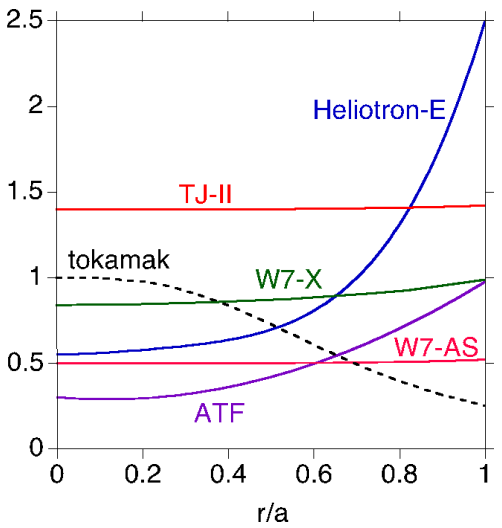
\includegraphics[scale=0.5]{img/compare.png}
    \caption[Perfiles radiales de transformada rotacional]{Perfiles radiales de transformada rotacional para diferentes
    conceptos de \textit{stellarators} y un \textit{tokamak}.}
    \label{fig:compare}
\end{figure}
Históricamente, los \textit{tokamaks} han utilizado el factor de seguridad $q=1/\iota$ y los stellarators $\iota$. En la figura~\ref{fig:compare} se muestran algunos perfiles de
transformada rotacional para diferentes \textit{stellarators} y un \textit{tokamak}. En un
\textit{tokamak} la corriente de plasma toroidal y por lo tanto, su contribución al 
campo magnético poloidal decrece con la distancia al centro; así la rotación
de las líneas de campo decrece. En un \textit{stellarator} el campo magnético poloidal
aumenta con la distancia al centro porque la contribución de las bobinas
exteriores helicoidales aumenta.\par
La cizalla magnética dada por 
\begin{equation}\label{eq:cizalla}
    s=-\frac{\rho}{\iota}\frac{d\iota}{d\rho}
\end{equation}
donde $\rho$ es radio normalizado efectivo del reactor, describe la variación
radial de la rotación de las líneas de campo magnético. Es obvio en la figura~\ref{fig:compare} que los \textit{stellarators} y los \textit{tokamaks} tienen signos opuestos de cizalla. Se
ha demostrado que las descargas de tokamak en las que se fuerza una cizalla
invertida, es decir, localmente este tipo de descargas tienen el mismo signo
de cizalla que un stellarator~\cite{PhysRevLett.75.4417}, a menudo tienen propiedades
de confinamiento mejorado en el plasma. TJ-II y W7-AS son \textit{stellarators}
con baja cizalla, mientras que LHD tiene una fuerte cizalla. Los
dispositivos con cizalla magnética tienen superficies de flujo con transformada
rotacional $\iota=n/m$, con $n$ y $m$ números naturales, llamados número toroidal
y número poloidal respectivamente. Este tipo de superficies de flujo se llaman
superficies racionales. Cuando m y n tienen valores pequeños, se
suelen llamar superficies racionales de bajo orden o simplemente racionales
de bajo orden. A modo de ejemplo, la superficie racional $\iota=8/5$,
se interpretaría geométricamente como: por cada $n=8$ vueltas poloidales la
línea de campo magnético daría $m=5$ vueltas toroidales. En una superficie
racional todas las líneas de campo son cerradas mientras que en una superficie
no racional las líneas de campo llenan la superficie magnética.
Existen inestabilidades que pueden producir que estas superficies
se destruyan localmente, dando origen a las llamadas islas magnéticas, esto son regiones del plasma donde las líneas llenan un volumen en vez de una
superficie y se hablara de ellas más adelante en este texto.
\subsection{Clasificación de los \textit{stellarators}}
Con respecto a la clasificación de los \textit{stellarators}, en la figura~\ref{fig:tree} se muestra la genealogía
de los distintos tipos de stellarators que han operado, operan o están en construcción. A
continuación se describen los principales:
\begin{itemize}
    \item \textit{Stellarator clásico}. Los stellarators clásicos constan de un grupo de bobinas planas circulares
    cuyos centros se encuentran en el mismo plano. Estas se encargan de producir
    el campo magnético toroidal. Un segundo grupo de $2l$ bobinas gira helicoidalmente $n$
    veces alrededor del plasma. La mitad de dichas bobinas helicoidales tiene la corriente
    en el sentido opuesto a la otra mitad de las bobinas. En la figura~\ref{fig:tree} se puede observar
    el stellarator \textit{Weldenstein 7-A} construido en Alemania con cuatro bobinas helicoidales
    $(l=2)$ que giran alrededor del plasma $n=5$ veces a lo largo de la dirección toroidal.
    Una de las ventajas de este tipo de \textit{stellarators} es que pueden variar el valor del campo
    toroidal y poloidal de manera independiente, lo cual permite variaciones en su transformada
    rotacional.
    Una de las desventajas de este tipo de stellarators son las fuerzas de interacción entre
    las bobinas toroidales y helicoidales.
    \item \textit{Torsatrón/Heliotrón}. Su construcción es similar a la de los stellarators clásicos. Se
    diferencian en que estos carecen de bobinas toroidales y la corriente que circula en
    las bobinas helicoidales tienen el mismo sentido. Estas generan en promedio un campo
    vertical que es compensado mediante bobinas circulares horizontales instaladas en la
    parte superior e inferior de la máquina. En la figura~\ref{fig:tree} se observa el torsatrón ATF
   $(l=2$ y $n=6)$, el cual ya no se encuentra en operativo. Otra máquina de este tipo
    que actualmente se encuentra en operación es el LHD $(l=2$ y $n=6)$ la cual cuenta con
    bobinas superconductoras para estudiar plasmas en estado estacionario.
    Una de las ventajas de esta configuración frente a los stellarators clásicos es que la
    ausencia de bobinas toroidales permite un mejor acceso al plasma por parte de los
    distintos diagnósticos.
    \item \textit{Heliacs}. Constan de un grupo de bobinas planas circulares que generan el campo
    magnético toroidal. Los centros de estas no están en el mismo plano, sino que describen
    una trayectoria helicoidal alrededor de un conductor central. Esta disposición de
    las bobinas, genera una geometría del campo magnético cuya sección poloidal tiene forma
    de alubia y cuyo eje magnético describe una trayectoria helicoidal alrededor
    de la bobina central. Máquinas representativas de esta configuración son TJ-II $(l=1$ y
    $n=4)$ y H-1 $(l=1$ y $n=3)$ en Australia.
    Debido a la flexibilidad que permiten este tipo de máquinas, son buenas candidatas
    para abordar estudios de estabilidad, equilibrio y transporte.
    \item \textit{Stellarator modular}. La característica fundamental de este tipo de \textit{stellarators} es que
    la forma geométrica de sus bobinas no es plana. Uno de los principales inconvenientes
    que presenta esta configuración es la fuerza de interacción entre las bobinas debido a la
    corta distancia entre ellas. Estas fuerzas suelen ser lo suficientemente elevadas como
    para provocar desplazamientos entre ellas. Por este motivo, conviene utilizar sujeciones
    mecánicas especiales en las bobinas.
    La principal ventaja de este tipo de máquinas reside en la variedad de configuraciones
    que puede adoptar. Ejemplos de máquinas con esta configuración son \textit{Weldenstein 7-AS},
    \textit{Weldenstein 7-X} ambas en Alemania y HSX en Estados Unidos.
\end{itemize}
\begin{figure}[H]
    \centering
    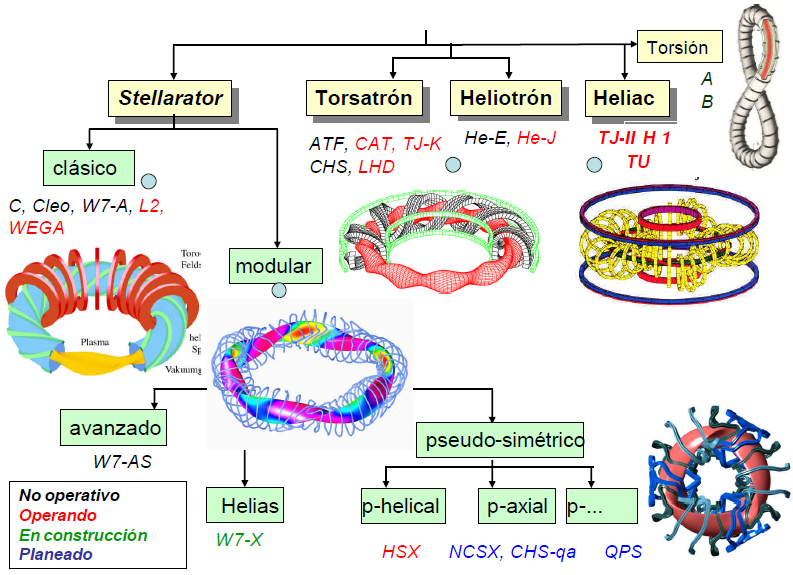
\includegraphics[scale=0.6]{img/tree.png}
    \caption[Diferentes conceptos de stellarator]{Diferentes conceptos de stellarator.}
    \label{fig:tree}
\end{figure}
\section{El \textit{stellarator} heliac flexible TJ-II}
Las características fundamentales del TJ-II~\cite{doi:10.13182/FST17-131-139} son:
\begin{enumerate}[(1)]
    \item Poseer el potencial suficiente para operar en regímenes de alta beta $(<\beta>\approx2\%)$.
    \item Tener una elevada flexibilidad magnética. Su transformada rotacional puede variar
    en un amplio rango.
    \item La sección poloidal del plasma tiene forma de alubia (configuración heliac).
\end{enumerate}
Podemos volver a definir $\beta$ de la ecuación~\eqref{eq:beta} como:
\begin{equation}\label{eq:beta2}
    \beta=\frac{(n_eT_E+n_iTi)k_B}{B^2/2\mu_0}
\end{equation}
donde $n_e$ y $n_i$ son la densidad electrónica e iónica respectivamente, $T_e$ y $T_i$ son la temperatura
electrónica e iónica, $k_B$ es la constante de Boltzmann, $\mu_0$ es la permeabilidad magnética en el
vacío y $B$ es el campo magnético.
En la tabla~\ref{tab:tj2} se resumen los parámetros fundamentales de la máquina. Posee 32 bobinas
que producen campo toroidal (TF), cuatro bobinas verticales que posicionan horizontalmente
el plasma (VF), una bobina circular (CC) y una bobina helicoidal $(l=1)$ (HX) que gira
en la dirección toroidal cuatro veces alrededor de la bobina circular, en cuatro períodos $(n=4)$; las dos bobinas CC y
HX constituyen el conductor central del dispositivo. La posibilidad de programar de manera
independiente la corriente que circula por estas dos bobinas es lo que proporciona el adjetivo
flexible a este dispositivo.
\begin{table}[H]
    \centering
    \begin{tabular}{cc}
    \hline
    PARÁMETRO & VALOR \\ \hline
    Número de períodos          & $n=4$       \\
    Número de bobinas TF          & 32       \\
    Radio mayor (m)          & $R_0=1.5$      \\
    Radio menor medio (m)          & $\langle a\rangle\leq 0.2$       \\
    Campo magnético (T)          & $B\leq 1$       \\
    Transformada rotacional          & $\iota(0)\approx0.9-2.2$       \\
    Densidad electrónica (ECRH) $(m^{-3})$          & $n^{ECRH}_{e,max}\approx 1.5\times 10^{19}$       \\
    Densidad electrónica (NBI) $(m^{-3})$          & $n^{NBI}_{e,max}\approx 8\times 10^{19}$       \\
    Temperatura electrónica máxima (keV)          & $T_e\approx 2$      \\
    Temperatura iónica (eV)          & $T_i\approx 150$      \\ \hline
    \end{tabular}
    \caption{Parámetros característicos del heliac flexible TJ-II.}
    \label{tab:tj2}
\end{table}
En la figura~\ref{fig:view} se muestra una vista en perspectiva del TJ-II.
\begin{figure}[h!]
    \centering
    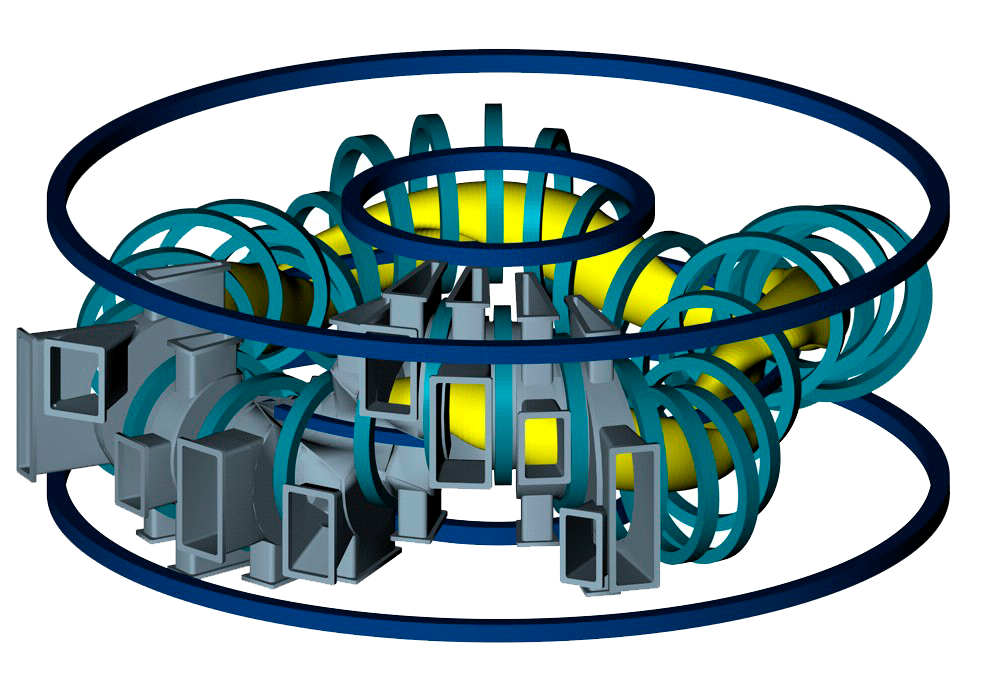
\includegraphics[height=4cm]{img/view.png}
    \caption[Vista en perspectiva del TJ-II]{Vista en perspectiva del TJ-II. En amarillo el plasma, en azul claro las bobinas toroidales y en azul oscuro, las radiales.}
    \label{fig:view}
\end{figure}
\subsection{Calentamiento del plasma}
Los plasmas utilizados en investigación de fusión nuclear poseen un alto grado de ionización 
para poder ser confinados magnéticamente. Para alcanzar esto, se ha de aportar energía al
gas inicial.
Para aportar energía al plasma, se pueden utilizar distintos mecanismos. En este texto se estudian
plasmas calentados mediante el sistema \textit{Neutral Beam Injector} (NBI) así como mediante
el sistema \textit{Electron Cyclotron Resonant Heating} (ECRH). A continuación, se describen
el funcionamiento y las características de ambos.
\subsubsection*{Calentamiento ECRH}
Este sistema se basa en
la aceleración de los electrones del plasma mediante haces de ondas electromagnéticas enfocadas
con altas densidades de potencia y cuya frecuencia es la de resonancia ciclotrónica de
los electrones.
Generalmente, estos sistemas constan de un girotrón donde se generan las ondas electromagnéticas, 
un camino óptico para transportar el haz de microondas hacia la cámara de
vacío y un espejo elipsoidal para enfocar el haz hacia el plasma.
En el camino óptico existen varios polarizadores, colocando estos de forma adecuada, se puede hacer que las ondas se propaguen
en el plasma de dos formas: el modo ordinario (modo-O) es aquel en el cual el campo
eléctrico de la onda es paralelo al campo magnético de la máquina o el modo extraordinario
(modo X), en el cual el campo eléctrico de la onda es perpendicular al campo magnético de
la máquina. La deposición de energía en el plasma mediante ECRH suele tener una buena localización
espacial, debido a que la frecuencia de resonancia de los electrones es función del valor de
campo magnético de la máquina, el cual varía a lo largo del radio. Uno de los usos que se le
da a esto es mitigar determinado
tipo de inestabilidades MHD~\cite{van_den_Brand_2012}.
El sistema de encendido y calentamiento del plasma mediante ECRH en el TJ-II consta de
dos girotrones operando en modo X a una frecuencia de 53.2 GHz que corresponde al segundo
armónico~\cite{Fernandez2001}. El calentamiento óptimo desde la zona de bajo campo se produce en el
primer armónico en modo O y en el segundo armónico en modo X. La elección de un modo
u otro depende entre otros aspectos del rango de densidades accesibles. Cada girotrón está diseñado
para proporcionar 300 kW de potencia de salida de microondas. El sistema posee dos líneas
que transmiten la potencia de las microondas al plasma mediante espejos, el último espejo
de cada línea está dentro de la cámara de vacío y permite variar el ángulo de lanzamiento
del haz de microondas y focalizarlo, consiguiéndose una alta eficiencia de absorción y una
estrecha deposición de la energía.
Uno de los inconvenientes del calentamiento ECRH es la densidad de corte, es decir, la densidad
del plasma a partir de la cual las ondas electromagnéticas se reflejan. Una futura máquina
de fusión tendrá dificultades para ser calentada únicamente mediante este método debido a
las altas densidades que se requieren en regiones centrales del plasma.
\subsubsection*{Calentamiento NBI}
El sistema de calentamiento NBI se basa en la inyección de un haz de neutros altamente
energético en el plasma, con ello no solo aumenta la temperatura electrónica e iónica, sino que
también lo hace la densidad de ambas especies. El motivo fundamental de que la inyección
sea de neutros es para que puedan penetrar en el plasma evitando interaccionar con el campo
magnético.
Una vez que el haz ha penetrado en el plasma, los neutros pueden ser ionizados por distintos
procesos atómicos tales como intercambio de carga, ionización por colisiones iónicas e
ionización por colisiones electrónicas. Una vez ionizados, estos son confinados por el campo
magnético de la máquina. Debido a la alta energía de los electrones y de los iones del haz,
es necesario que el campo magnético de la máquina sea lo suficientemente intenso como para
confinarlos.
Los iones provenientes del haz son más energéticos que los electrones debido a su diferencia de
masa, los primeros comienzan a ser frenados debido a las colisiones Culombianas con iones
y electrones del plasma. En esas colisiones tiene lugar la transferencia de energía de los iones
provenientes del haz a los iones y electrones presentes en el plasma.\par
En lo que respecta a la posición en la que se han de ionizar los neutros, conviene que el
proceso tenga lugar en el centro de la columna de plasma, para ello existe un compromiso
entre la densidad del plasma y la energía del haz. Si el plasma es poco denso o el haz muy
energético podría no producirse ionización, lo que conduciría a que muchos neutros impactaran
en la pared con su consecuente deterioro. Si por el contrario el plasma es muy denso
o el haz poco energético, entonces los neutros se ionizarían justo en el borde del plasma, lo
que provocaría un pico en la densidad del borde que lleva a una inestabilidad del plasma.
En lo referente a la forma en la que se inyectan los neutros en la cámara existen fundamentalmente
tres formas: inyección co-tangencial, en la cual los neutros son inyectados paralelamente
al campo magnético y a favor de la corriente de la máquina; inyección contra-tangencial, en
la cual los neutros son inyectados en contra de la corriente de la máquina y por último existe
la inyección perpendicular a las líneas de campo magnético. Las tres formas que se han mencionado
producen un incremento de la temperatura electrónica y/o iónica en el plasma, pero
solo las dos primeras producen una corriente o un momento en el sentido de la inyección~\cite{wesson2004tokamaks}.
El sistema NBI instalado en TJ-II, es capaz de inyectar una potencia que varía de 1 a 1.5
MW. Dicho sistema posee dos líneas de calentamiento, una co-tangencial y la otra contratangencial.
Una desventaja de los sistemas NBI es el tamaño del equipo, sin embargo, tienen la ventaja
de que pueden ser probados independientemente de la máquina. Otra desventaja desde el
punto de vista de un reactor de fusión es que el sistema de calentamiento NBI ha de estar
muy cerca del plasma por lo que sufrirá flujos neutrónicos y contaminación por Tritio.